%! TeX root = ../root/root.tex 
\section{Resultados}

\subsection{Vacâncias No Cristal Volumoso}
\begin{frame}[allowframebreaks]{Densidade de Estados Projetada -- Defeitos Neutros}
	\begin{figure}[t]
		\centering
		\includegraphics{../floats/pdos_vac/pdos_neutral_d_separated_333_vO.pdf}
		\caption{pDOS do v$_{\ce{O}}^0$ na supercélula $3\times3\times3$. Linha tracejada indica o nivel de Fermi ($\varepsilon_F$).\label{fig:pdosNeuVac_vO}}
	\end{figure}
	\begin{itemize}
		\item Átomo de \ce{O} removido $\to$ redução no nível energético de \ce{Nb} $4d_{3z^2-r^2}$ $+$ preenchimento parcial $\to$ \alert{níveis rasos doadores};
		\begin{itemize}
			\item \ce{O} apical removido $\to$ quebra da degenerescência $e_g$ $\to$ níveis \ce{Nb} $4d_{3z^2-r^2}$ abaixam ao remover a sobreposição de orbitais $p-d$;
			\item Nível de defeito \SI{27}{\milli\electronvolt} abaixo da condução $\to$ perto de ionizar com energia térmica ($300 k_B \approx \SI{26}{\milli\electronvolt}$);
			\item Pode haver \alert{aumento da densidade de elétrons} sem grande impacto à condutividade $\to$ melhora na reação de evolução de hidrogênio;
		\end{itemize}
	\end{itemize}\framebreak
	\begin{figure}[t]
		\centering
		\includegraphics{../floats/pdos_vac/pdos_neutral_d_separated_333_vNa.pdf}
		\caption{pDOS do v$_{\ce{Na}}^0$ na supercélula $3\times3\times3$. Linha tracejada indica o nivel de Fermi ($\varepsilon_F$).\label{fig:pdosNeuVac_vNa}}
	\end{figure}
	\begin{itemize}
		\item Átomo de \ce{Na} removido $\to$ aumento do nível energético de \ce{O} $2p$ $+$ depleção parcial $\to$ \alert{níveis rasos aceitadores};
		\begin{itemize}
			\item Quebra de ligações \ce{Na-O} $\to$ orbitais \ce{O} $2p$ parcialmente preenchidos;
			\item Nível de defeito \SI{10}{\milli\electronvolt} acima da valência $\to$ ionização por energia térmica permitida;
			\item Pode haver \alert{aumento da densidade de lacunas} sem grande impacto na condutividade $\to$ melhora na reação de evolução de oxigênio;
		\end{itemize}
	\end{itemize}\framebreak
\end{frame}
\begin{frame}{Estrutura Cristalina}
	\begin{figure}[htb]
		\centering
		\input{../floats/geometry_vac/neighborhood_o0.pdf_tex}
		\caption{O arranjo atômico maios próximo ao defeito pontual antes (esquerda) e depois (direita) de formado. Após relaxação atômica, os \ce{O} (vermelho) equatoriais se aproximam do defeito enquanto os \ce{Nb} se afastam. Os ângulos \ce{Nb-O-Nb} dos \ce{O} equatoriais diminuem.}
	\end{figure}
	\begin{itemize}
		\item Vacância de \ce{O}: \ce{Nb} vizinhos se aproximam dos \ce{O} que formam o \ce{NbO5} compensando elétrons na valência do \ce{Nb};
		\item Vacância de \ce{Na}: preservação da disposição atômica anterior ao defeito pontual;
		\item Intensidade das ligações \ce{Nb-O} \textit{vs.} \ce{Na-O};
	\end{itemize}
\end{frame}
\begin{frame}[allowframebreaks]{Densidade De Estados Projetada -- Defeitos Com Carga}
	\begin{figure}[t]
		\centering
		\includegraphics[scale=1]{../floats/pdos_vac/pdos_charged_d_separated_333.pdf}
		\caption{pDOS com v$_{\ce{O}}^{2+}$ e com v$_{\ce{Na}}^{1-}$ em supercélulas $3\times3\times3$. Linha tracejada indica o nivel de Fermi ($\varepsilon_F$).\label{fig:pdosChaVac}}
	\end{figure}\framebreak
	\begin{itemize}
		\item Ionização pouco altera a distância dos níveis energéticos de defeito pontial em relação aos limites de banda;
		\item Níveis de defeito do v${}_{\ce{O}}^{2+}$ esvaziados;
		\item Níveis de defeito do v${}_{\ce{Na}}^{1-}$ preenchidos;
		\item Tamanho da banda proibida: de \SI{1.91}{\electronvolt} foi para \SI{1.95}{\electronvolt} com v$_{\ce{O}}^{2+}$ e \SI{1.96}{\electronvolt} com v$_{\ce{Na}}^{1-}$;
		\begin{itemize}
			\item Níveis de defeito deveriam \alert{reduzir} a banda proibida;
			\item Banda proibida depende da repulsão dos orbitais $p-d$ ao serem sobrepostos na ligação \ce{Nb-O};
			\item DFT superestima delocalização de orbitais $d$ $\to$ imprecisão na descrição da sobreposição $p-d$;
			\item Comportamento se mantém com melhor descrição dos orbitais $d$ ou da energia de troca e correlação?
		\end{itemize}
	\end{itemize}
\end{frame}
\begin{frame}{Energia de Formação: \texorpdfstring{v$_{\ce{Na}}^{0}$}{vNa0}}
	\begin{columns}
		\begin{column}{.5\textwidth}
			\begin{figure}[t]
				\centering
				\begin{tikzpicture}
    \begin{ternaryaxis}[
        width=0.82\textwidth,
        xlabel=O ($\%$),
        xlabel style={%
            font=\footnotesize,
            at={(axis cs:1,0,0)},
            anchor=south
        },
        xtick={0.2,0.4,0.6,0.8},
        xticklabels={$20$,$40$,$60$,$80$},
        xticklabel style={font=\footnotesize},
        xtick style={line width=0.25mm, color=black},
        ylabel=Na ($\%$),
        ylabel style={%
            font=\footnotesize,
            at={(axis cs:0,1,0)},
            anchor=north,
            rotate=-60
        },
        ytick={0.2,0.4,0.6,0.8},
        yticklabels={$20$,$40$,$60$,$80$},
        yticklabel style={font=\footnotesize},
        ytick style={line width=0.25mm, color=black},
        zlabel=Nb ($\%$),
        zlabel style={%
            font=\footnotesize,
            at={(axis cs:0,0,1)},
            anchor=north,
            rotate=60
        },
        ztick={0.2,0.4,0.6,0.8},
        zticklabels={$20$,$40$,$60$,$80$},
        zticklabel style={font=\footnotesize},
        ztick style={line width=0.25mm, color=black},
        clip=false,
        no markers,
        colorbar,
        colormap/bluered,
        colorbar style={%
            ylabel=$\Delta E_f (\text{v}_{\ce{X}}^{q}; L\to\infty)$ (\si{\electronvolt}),
            ylabel style={
                font=\footnotesize,
                at={(axis description cs:5.0,0.5)}
            },
            yticklabel style={%
                font=\footnotesize,
                /pgf/number format/.cd,
                fixed,
                fixed zerofill,
                precision=0,
                /tikz/.cd
            },
            ytick style={line width=0.25mm, color=black},
        },
        point meta min=-2.0,
        of colormap/target pos min*=-2.0,
        point meta max=6.9814,
        of colormap/target pos max*=6.9814
    ]
        \addplot3 [patch, faceted color=black, point meta=\thisrow{H}] table {%
            O        Na       Nb       H
            1.0      0.0      0.0      3.4040
            0.6      0.2      0.2      3.4040
            0.666667 0.333333 0.0      3.4040
        };

        \addplot3 [patch, faceted color=black, point meta=\thisrow{H}] table {%
            O        Na       Nb       H
            0.666667 0.333333 0.0      3.5950
            0.6      0.2      0.2      3.5950
            0.5      0.5      0.0      3.5950
        };

        \addplot3 [patch, faceted color=black, point meta=\thisrow{H}] table {%
            O        Na       Nb       H
            0.5      0.5      0.0      4.1621
            0.6      0.2      0.2      4.1621
            0.333333 0.666667 0.0      4.1621
        };

        \addplot3 [patch, faceted color=black, point meta=\thisrow{H}] table {%
            O        Na       Nb       H
            0.333333 0.666667 0.0      5.6681
            0.6      0.2      0.2      5.6681
            0.0      1.0      0.0      5.6681
        };

        \addplot3 [patch, faceted color=black, point meta=\thisrow{H}] table {%
            O        Na       Nb       H
            0.0      1.0      0.0      5.6681
            0.6      0.2      0.2      5.6681
            0.0      0.0      1.0      5.6681
        };

        \addplot3 [patch, faceted color=black, point meta=\thisrow{H}] table {%
            O        Na       Nb       H
            0.0      0.0      1.0      5.2642
            0.6      0.2      0.2      5.2642
            0.5      0.0      0.5      5.2642
        };

        \addplot3 [patch, faceted color=black, point meta=\thisrow{H}] table {%
            O        Na       Nb       H
            0.5      0.0      0.5      4.3482
            0.6      0.2      0.2      4.3482
            0.666667 0.0      0.333333 4.3482
        };

        \addplot3 [patch, faceted color=black, point meta=\thisrow{H}] table {%
            O        Na       Nb       H
            0.714286 0.0      0.285714 4.0844
            0.6      0.2      0.2      4.0844
            0.666667 0.0      0.333333 4.0844
        };

        \addplot3 [patch, faceted color=black, point meta=\thisrow{H}] table {%
            O        Na       Nb       H
            0.714286 0.0      0.285714 2.4897
            0.6      0.2      0.2      2.4897
            1.0      0.0      0.0      2.4897
        };

        \node [] at (cartesian cs:0.450, 0.650) {\footnotesize A};
        \node [] at (cartesian cs:0.350, 0.510) {\footnotesize B};
        \node [] at (cartesian cs:0.275, 0.400) {\footnotesize C};
        \node [] at (cartesian cs:0.200, 0.265) {\footnotesize \textcolor{white}{D}};
        \node [] at (cartesian cs:0.500, 0.200) {\footnotesize \textcolor{white}{E}};
        \node [] at (cartesian cs:0.701, 0.375) {\footnotesize \textcolor{white}{F}};
        \node [] at (cartesian cs:0.650, 0.510) {\footnotesize G};
        \node [pin={[pin distance=7ex, pin edge={black, thick}]15:\footnotesize H}] at (cartesian cs:0.600, 0.570) {};
        \node [] at (cartesian cs:0.550, 0.650) {\footnotesize I};
        \node [] at (cartesian cs:0.000, 0.920) {v$_{\ce{Na}}^0$};
    \end{ternaryaxis}
\end{tikzpicture}

				\caption{Variação do $\Delta E_f (\text{v}_{\ce{Na}}^{0};\, L \to \infty)$ em função do equilíbrio químico.\label{fig:energy_vac_na0}}
			\end{figure}
		\end{column}
		\begin{column}{.5\textwidth}
			\begin{itemize}
				\item Mínimo de \SI{2.49}{\electronvolt} com eq. \ce{Nb2O5-NaNbO3-O} (I) $\to$ favorecimento em condições oxidantes;
				\begin{itemize}
					\item Problema de volatividade do \ce{Na}\footnote[frame]{\cite{acker_microstructure_2014}};
				\end{itemize}
				\item $\Delta E_f$ cresce com o caráter redutor;
			\end{itemize}
		\end{column}
	\end{columns}
\end{frame}
\begin{frame}{Energia de Formação: \texorpdfstring{v$_{\ce{O}}^{0}$}{vO0}}
	\begin{columns}
		\begin{column}{.5\textwidth}
			\begin{figure}[t]
				\centering
				\begin{tikzpicture}
    \begin{ternaryaxis}[
        width=0.82\textwidth,
        xlabel=O ($\%$),
        xlabel style={%
            font=\footnotesize,
            at={(axis cs:1,0,0)},
            anchor=south
        },
        xtick={0.2,0.4,0.6,0.8},
        xticklabels={$20$,$40$,$60$,$80$},
        xticklabel style={font=\footnotesize},
        xtick style={line width=0.25mm, color=black},
        ylabel=Na ($\%$),
        ylabel style={%
            font=\footnotesize,
            at={(axis cs:0,1,0)},
            anchor=north,
            rotate=-60
        },
        ytick={0.2,0.4,0.6,0.8},
        yticklabels={$20$,$40$,$60$,$80$},
        yticklabel style={font=\footnotesize},
        ytick style={line width=0.25mm, color=black},
        zlabel=Nb ($\%$),
        zlabel style={%
            font=\footnotesize,
            at={(axis cs:0,0,1)},
            anchor=north,
            rotate=60
        },
        ztick={0.2,0.4,0.6,0.8},
        zticklabels={$20$,$40$,$60$,$80$},
        zticklabel style={font=\footnotesize},
        ztick style={line width=0.25mm, color=black},
        clip=false,
        no markers,
        colorbar,
        colormap/bluered,
        colorbar style={%
            ylabel=$\Delta E_f (\text{v}_{\ce{X}}^{q}; L\to\infty)$ (\si{\electronvolt}),
            ylabel style={
                font=\footnotesize,
                at={(axis description cs:5.0,0.5)}
            },
            yticklabel style={%
                font=\footnotesize,
                /pgf/number format/.cd,
                fixed,
                fixed zerofill,
                precision=0,
                /tikz/.cd
            },
            ytick style={line width=0.25mm, color=black},
        },
        point meta min=-2.0,
        of colormap/target pos min*=-2.0,
        point meta max=6.9814,
        of colormap/target pos max*=6.9814
    ]
        \addplot3 [patch, faceted color=black, point meta=\thisrow{H}] table {%
            O        Na       Nb       H
            1.0      0.0      0.0      5.3183
            0.6      0.2      0.2      5.3183
            0.666667 0.333333 0.0      5.3183
        };

        \addplot3 [patch, faceted color=black, point meta=\thisrow{H}] table {%
            O        Na       Nb       H
            0.666667 0.333333 0.0      5.2228
            0.6      0.2      0.2      5.2228
            0.5      0.5      0.0      5.2228
        };

        \addplot3 [patch, faceted color=black, point meta=\thisrow{H}] table {%
            O        Na       Nb       H
            0.5      0.5      0.0      4.6557
            0.6      0.2      0.2      4.6557
            0.333333 0.666667 0.0      4.6557
        };

        \addplot3 [patch, faceted color=black, point meta=\thisrow{H}] table {%
            O        Na       Nb       H
            0.333333 0.666667 0.0      1.6438
            0.6      0.2      0.2      1.6438
            0.0      1.0      0.0      1.6438
        };

        \addplot3 [patch, faceted color=black, point meta=\thisrow{H}] table {%
            O        Na       Nb       H
            0.0      1.0      0.0      1.2724
            0.6      0.2      0.2      1.2724
            0.0      0.0      1.0      1.2724
        };

        \addplot3 [patch, faceted color=black, point meta=\thisrow{H}] table {%
            O        Na       Nb       H
            0.0      0.0      1.0      1.4071
            0.6      0.2      0.2      1.4071
            0.5      0.0      0.5      1.4071
        };

        \addplot3 [patch, faceted color=black, point meta=\thisrow{H}] table {%
            O        Na       Nb       H
            0.5      0.0      0.5      1.8651
            0.6      0.2      0.2      1.8651
            0.666667 0.0      0.333333 1.8651
        };

        \addplot3 [patch, faceted color=black, point meta=\thisrow{H}] table {%
            O        Na       Nb       H
            0.714286 0.0      0.285714 2.1288
            0.6      0.2      0.2      2.1288
            0.666667 0.0      0.333333 2.1288
        };

        \addplot3 [patch, faceted color=black, point meta=\thisrow{H}] table {%
            O        Na       Nb       H
            0.714286 0.0      0.285714 5.3183
            0.6      0.2      0.2      5.3183
            1.0      0.0      0.0      5.3183
        };

        \node [] at (cartesian cs:0.450, 0.650) {\footnotesize\textcolor{white}{A}};
        \node [] at (cartesian cs:0.350, 0.510) {\footnotesize\textcolor{white}{B}};
        \node [] at (cartesian cs:0.275, 0.400) {\footnotesize\textcolor{white}{C}};
        \node [] at (cartesian cs:0.200, 0.265) {\footnotesize D};
        \node [] at (cartesian cs:0.500, 0.200) {\footnotesize E};
        \node [] at (cartesian cs:0.701, 0.375) {\footnotesize F};
        \node [] at (cartesian cs:0.650, 0.510) {\footnotesize G};
        \node [pin={[pin distance=7ex, pin edge={black, thick}]15:\footnotesize H}] at (cartesian cs:0.600, 0.570) {};
        \node [] at (cartesian cs:0.550, 0.650) {\footnotesize\textcolor{white}{I}};
        \node [] at (cartesian cs:0.000, 0.920) {v$_{\ce{O}}^0$};
    \end{ternaryaxis}
\end{tikzpicture}

				\caption{Variação do $\Delta E_f (\text{v}_{\ce{O}}^{0};\, L \to \infty)$ em função do equilíbrio químico.\label{fig:energy_vac_o0}}
			\end{figure}
		\end{column}
		\begin{column}{.5\textwidth}
			\begin{itemize}
				\item Mínimo de \SI{1.27}{\electronvolt} com equilíbrio \ce{Na-NaNbO3-Nb} (E) $\to$ favorecimento em condições redutoras;
				\item $\Delta E_f$ cresce com o caráter oxidante;
			\end{itemize}
			\begin{center}
				\alert{Ambientes mais redutores que em C e H favorecem v$_{\ce{O}}^{0}$ em detrimento de v$_{\ce{Na}}^{0}$!}
			\end{center}
		\end{column}
	\end{columns}
\end{frame}
\begin{frame}{Energia de Formação: \texorpdfstring{v$_{\ce{Na}}^{1-}$}{vNa1-}}
	\begin{columns}
		\begin{column}{.5\textwidth}
			\begin{figure}[t]
				\centering
				\input{../floats/energy_vac/hvac_na1}
				\caption{Variação do $\Delta E_f (\text{v}_{\ce{Na}}^{1-};\, L \to \infty)$ em função do equilíbrio químico.\label{fig:energy_vac_na1}}
			\end{figure}
		\end{column}
		\begin{column}{.5\textwidth}
			\begin{itemize}
				\item Mínimo de \SI{3.80}{\electronvolt} com eq. \ce{Nb2O5-NaNbO3-O} (I) $\to$ favorecimento em condições oxidantes;
				\item $\Delta E_f (\text{v}_{\ce{Na}}^{1-}) > \Delta E_f (\text{v}_{\ce{Na}}^{0}) \to$ formação do defeito pontual neutro;
			\end{itemize}
		\end{column}
	\end{columns}
\end{frame}
\begin{frame}{Energia de Formação: \texorpdfstring{v$_{\ce{O}}^{2+}$}{vO2+} I}
	\begin{columns}
		\begin{column}{.5\textwidth}
			\begin{figure}[t]
				\centering
				\begin{tikzpicture}
    \begin{ternaryaxis}[
        width=.82\textwidth,
        xlabel=O ($\%$),
        xlabel style={%
            font=\footnotesize,
            at={(axis cs:1,0,0)},
            anchor=south
        },
        xtick={0.2,0.4,0.6,0.8},
        xticklabels={$20$,$40$,$60$,$80$},
        xticklabel style={font=\footnotesize},
        xtick style={line width=0.25mm, color=black},
        ylabel=Na ($\%$),
        ylabel style={%
            font=\footnotesize,
            at={(axis cs:0,1,0)},
            anchor=north,
            rotate=-60
        },
        ytick={0.2,0.4,0.6,0.8},
        yticklabels={$20$,$40$,$60$,$80$},
        yticklabel style={font=\footnotesize},
        ytick style={line width=0.25mm, color=black},
        zlabel=Nb ($\%$),
        zlabel style={%
            font=\footnotesize,
            at={(axis cs:0,0,1)},
            anchor=north,
            rotate=60
        },
        ztick={0.2,0.4,0.6,0.8},
        zticklabels={$20$,$40$,$60$,$80$},
        zticklabel style={font=\footnotesize},
        ztick style={line width=0.25mm, color=black},
        clip=false,
        no markers,
        colorbar,
        colormap/bluered,
        colorbar style={%
            ylabel=$\Delta E_f (\text{v}_{\ce{X}}^{q}; L\to\infty)$ (\si{\electronvolt}),
            ylabel style={
                font=\footnotesize,
                at={(axis description cs:5.0,0.5)}
            },
            yticklabel style={%
                font=\footnotesize,
                /pgf/number format/.cd,
                fixed,
                fixed zerofill,
                precision=0,
                /tikz/.cd
            },
            ytick style={line width=0.25mm, color=black},
        },
        point meta min=-2.0,
        of colormap/target pos min*=-2.0,
        point meta max=6.9814,
        of colormap/target pos max*=6.9814
    ]
        \addplot3 [patch, faceted color=black, point meta=\thisrow{H}] table {%
            O        Na       Nb       H
            1.0      0.0      0.0      2.0927
            0.6      0.2      0.2      2.0927
            0.666667 0.333333 0.0      2.0927
        };

        \addplot3 [patch, faceted color=black, point meta=\thisrow{H}] table {%
            O        Na       Nb       H
            0.666667 0.333333 0.0      1.9972
            0.6      0.2      0.2      1.9972
            0.5      0.5      0.0      1.9972
        };

        \addplot3 [patch, faceted color=black, point meta=\thisrow{H}] table {%
            O        Na       Nb       H
            0.5      0.5      0.0      1.4301
            0.6      0.2      0.2      1.4301
            0.333333 0.666667 0.0      1.4301
        };

        \addplot3 [patch, faceted color=black, point meta=\thisrow{H}] table {%
            O        Na       Nb       H
            0.333333 0.666667 0.0      -1.5818
            0.6      0.2      0.2      -1.5818
            0.0      1.0      0.0      -1.5818
        };

        \addplot3 [patch, faceted color=black, point meta=\thisrow{H}] table {%
            O        Na       Nb       H
            0.0      1.0      0.0      -1.9532
            0.6      0.2      0.2      -1.9532
            0.0      0.0      1.0      -1.9532
        };

        \addplot3 [patch, faceted color=black, point meta=\thisrow{H}] table {%
            O        Na       Nb       H
            0.0      0.0      1.0      -1.8185
            0.6      0.2      0.2      -1.8185
            0.5      0.0      0.5      -1.8185
        };

        \addplot3 [patch, faceted color=black, point meta=\thisrow{H}] table {%
            O        Na       Nb       H
            0.5      0.0      0.5      -1.3605
            0.6      0.2      0.2      -1.3605
            0.666667 0.0      0.333333 -1.3605
        };

        \addplot3 [patch, faceted color=black, point meta=\thisrow{H}] table {%
            O        Na       Nb       H
            0.714286 0.0      0.285714 -1.0968
            0.6      0.2      0.2      -1.0968
            0.666667 0.0      0.333333 -1.0968
        };

        \addplot3 [patch, faceted color=black, point meta=\thisrow{H}] table {%
            O        Na       Nb       H
            0.714286 0.0      0.285714 2.0927
            0.6      0.2      0.2      2.0927
            1.0      0.0      0.0      2.0927
        };

        \node [] at (cartesian cs:0.450, 0.650) {\footnotesize A};
        \node [] at (cartesian cs:0.350, 0.510) {\footnotesize B};
        \node [] at (cartesian cs:0.275, 0.400) {\footnotesize C};
        \node [] at (cartesian cs:0.200, 0.265) {\footnotesize\textcolor{white}{D}};
        \node [] at (cartesian cs:0.500, 0.200) {\footnotesize\textcolor{white}{E}};
        \node [] at (cartesian cs:0.701, 0.375) {\footnotesize\textcolor{white}{F}};
        \node [] at (cartesian cs:0.650, 0.510) {\footnotesize\textcolor{white}{G}};
        \node [pin={[pin distance=7ex, pin edge={black, thick}]15:\footnotesize H}] at (cartesian cs:0.600, 0.570) {};
        \node [] at (cartesian cs:0.550, 0.650) {\footnotesize I};
        \node [] at (cartesian cs:0.000, 0.920) {v$_{\ce{O}}^{2+}$};
    \end{ternaryaxis}
\end{tikzpicture}

				\caption{Variação do $\Delta E_f (\text{v}_{\ce{O}}^{2+};\, L \to \infty)$ em função do equilíbrio químico.\label{fig:energy_vac_o2}}
			\end{figure}
		\end{column}
		\begin{column}{.5\textwidth}
			\begin{itemize}
				\item Mínimo de \SI{-1.95}{\electronvolt} com equilíbrio \ce{Na-NaNbO3-Nb} (E) $\to$ favorecimento em condições redutoras;
				\item $\Delta E_f (\text{v}_{\ce{O}}^{2+}) << \Delta E_f (\text{v}_{\ce{O}}^{0}) \to$ formação do defeito pontual ionizado;
				\item \alert{Energias de formação negativas para equilíbrios químicos entre D e H;}
			\end{itemize}
		\end{column}
	\end{columns}
\end{frame}
\begin{frame}{Energia de Formação: \texorpdfstring{v$_{\ce{O}}^{2+}$}{vO2+} II}
	\begin{itemize}
		\item $\Delta E_f (\text{v}_{\ce{O}}^{2+}; L) < 0$ para os três tamanhos de supercélula $\to$ $\Delta E_f (\text{v}_{\ce{O}}^{2+}; L \to \infty) < 0$;
		\item Fatores:
		\begin{itemize}
			\item $E_T (\text{v}_{\ce{O}}^{2+}; L) - E_T (\text{perfeito}; L) > 0$ para $1\times1\times1$, $2\times2\times2$ e $3\times3\times3$;
			\item $E_T (\text{v}_{\ce{O}}^{2+}; L) - E_T (\text{perfeito}; L) + q \varepsilon_F > 0$ para todas as supercélulas;
			\item $E_T (\text{v}_{\ce{O}}^{2+}; L) - E_T (\text{perfeito}; L) + q \varepsilon_F < | \mu_{\ce{O}} |$ para os equilíbrios D à H;
		\end{itemize}
		\item Hipótese: $E_T (\text{v}_{\ce{O}}^{2+}; L) - E_T (\text{perfeito}; L)$ ou $ q \varepsilon_F$ subestimados $\to$ troca com reservatório $e^{-}$ depende do tamanho de banda proibida;
		\begin{itemize}
			\item $q \varepsilon_F$ da banda proibida experimental\footnote[frame]{\cite{li_constructing_2014}} (\SI{3.42}{\electronvolt}) dá $\Delta E_f (\text{v}_{\ce{O}}^{2+}; L \to \infty) = \SI{0.08}{\electronvolt}$ $\to$ melhor descrição da banda proibida pode melhorar a descrição de v$_{\ce{O}}^{2+}$;
			\item Modelo de v$_{\ce{O}}^{2+}$ isolado? Modelo com um defeito de Schottky/Frenkel?
		\end{itemize}\vfill
		\begin{equation*}
			\Delta E_f (\text{v}_{\ce{X}}^{q}; L) = E_T (\text{v}_{\ce{X}}^{q}; L) - E_T (\text{perfeito}; L) - n_{\ce{X}} \mu_{\ce{X}} + q \varepsilon_F + E_c
		\end{equation*}
	\end{itemize}
\end{frame}

\subsection{Filme Fino De \texorpdfstring{\ce{NaNbO3}}{NaNbO3} Orientado Em \texorpdfstring{$[100]$}{[100]}}
\begin{frame}{Reconfiguração Cristalina}
	\begin{columns}
		\begin{column}{.4\textwidth}
			\begin{figure}[t]
				\centering
				%! TeX root = ../root/root.tex 
\begin{tikzpicture}[remember picture, baseline=-.5ex]
    \draw (0.00cm, 0.00cm) node {
        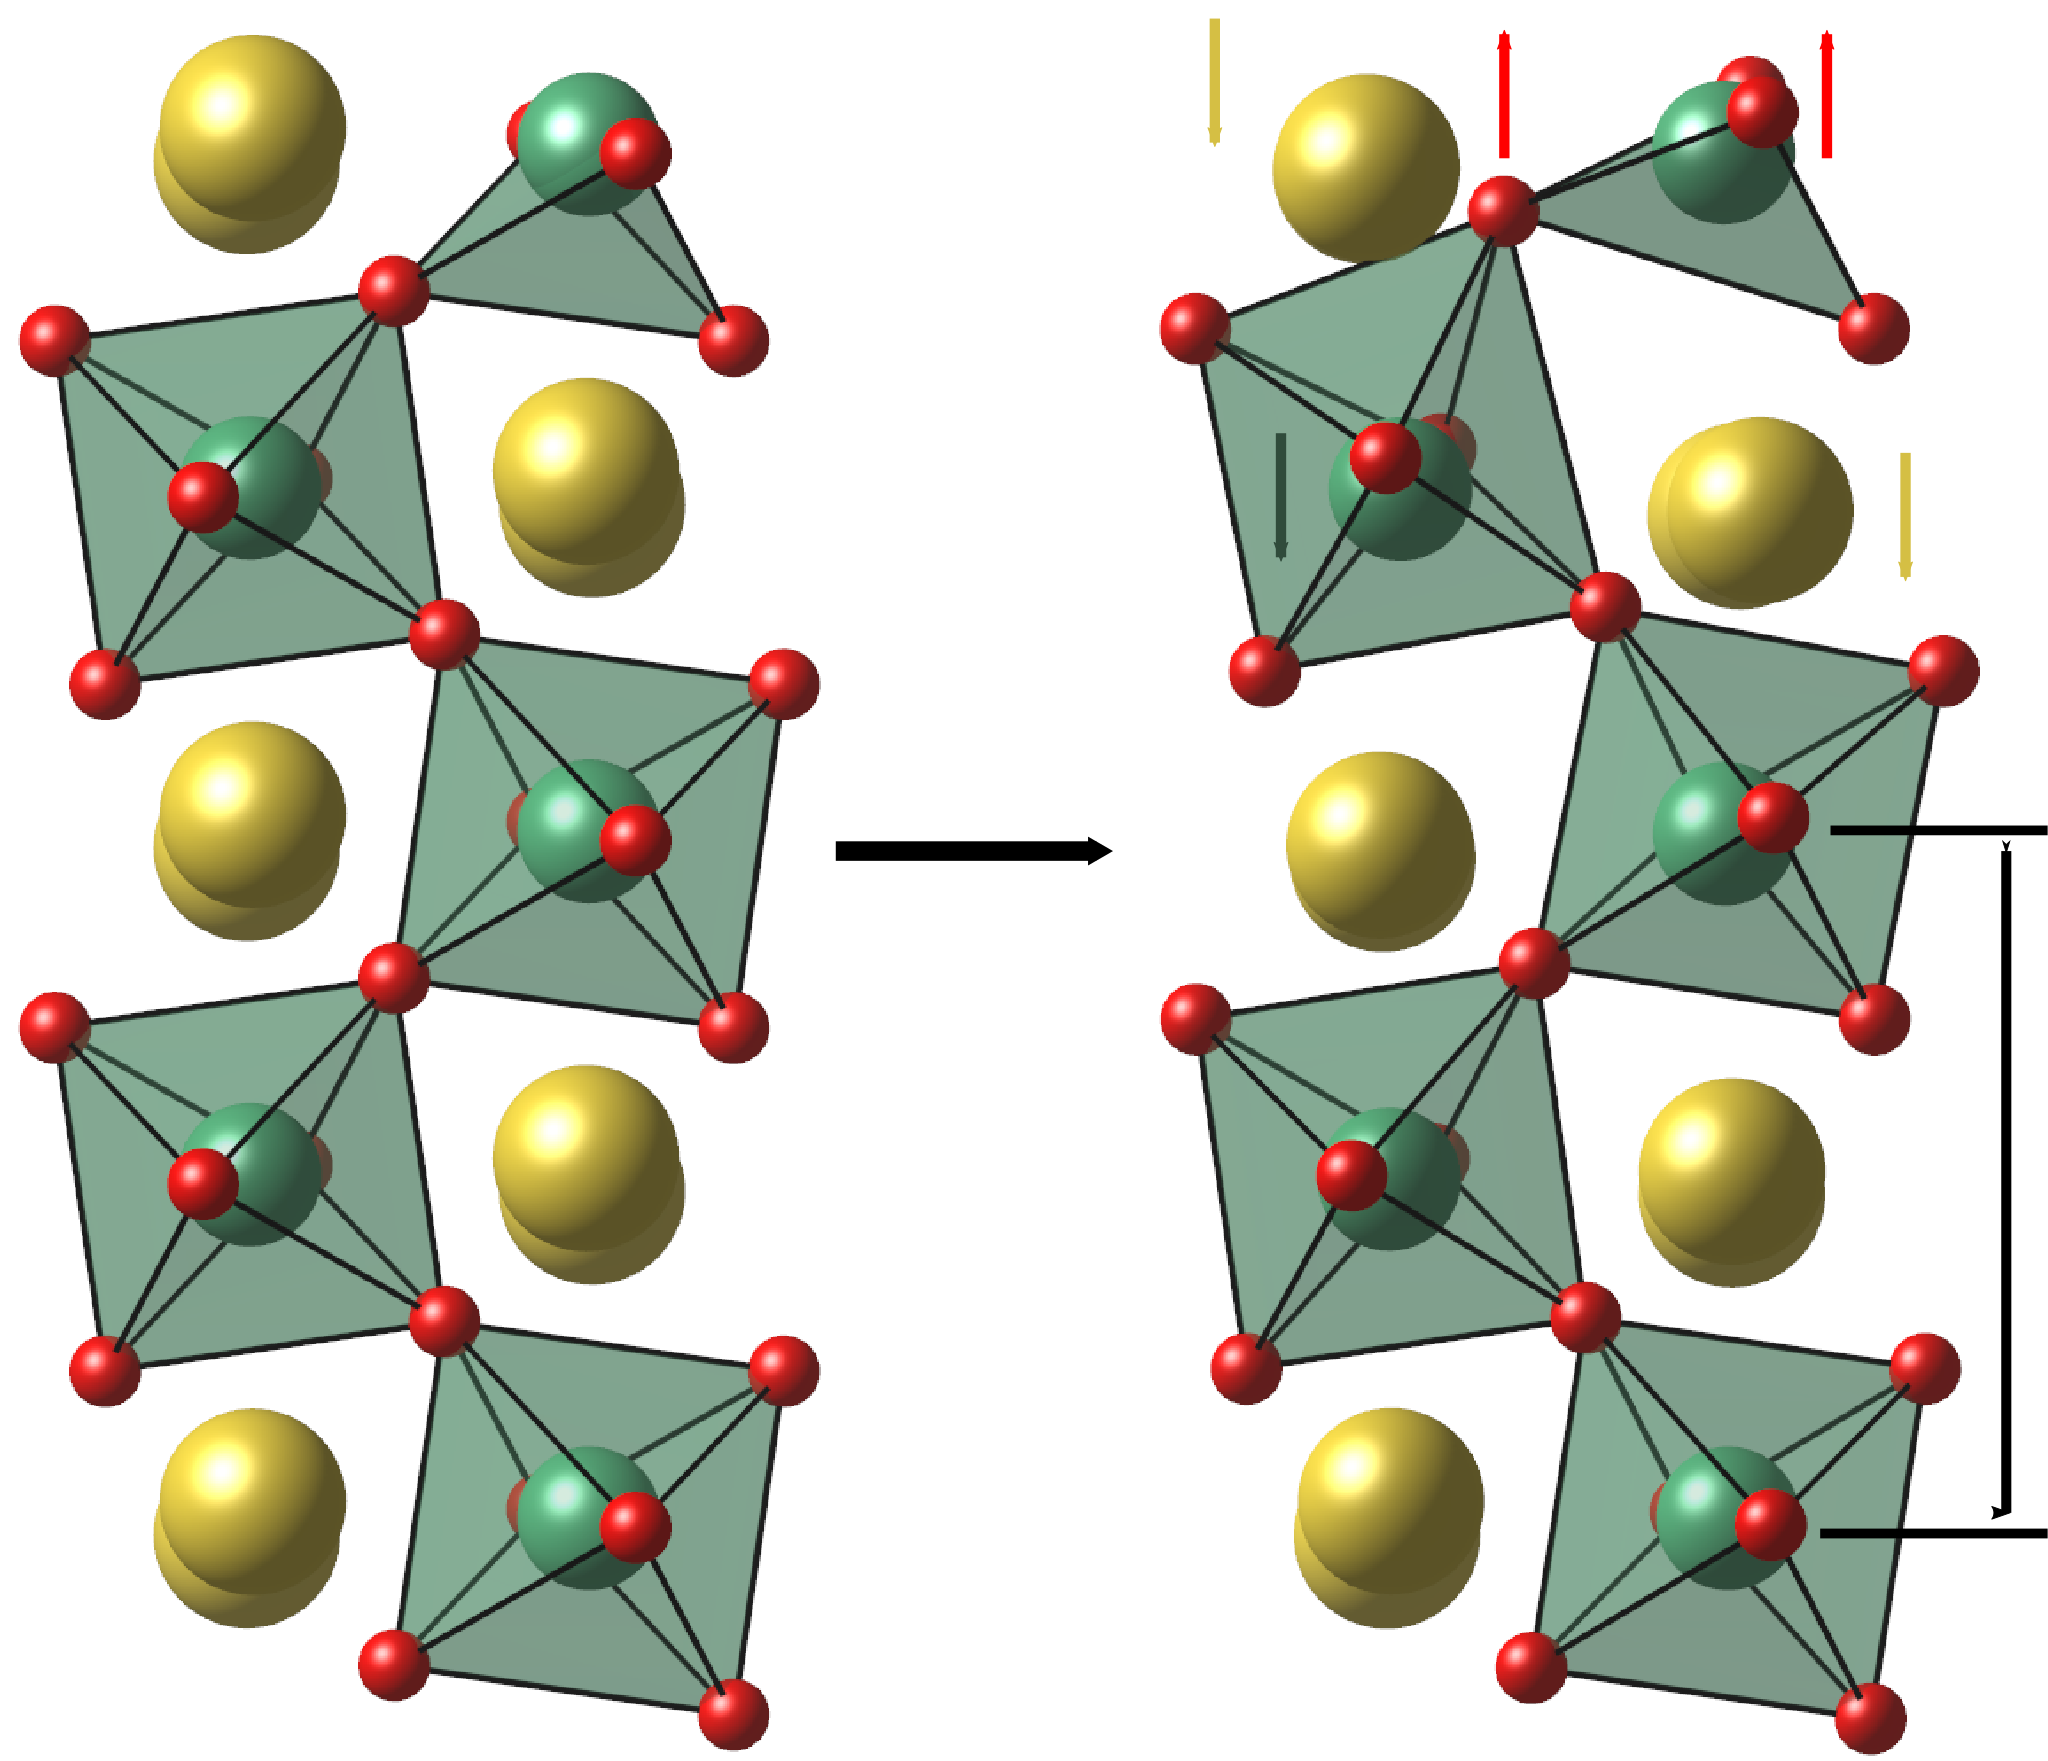
\includegraphics[width=0.85\linewidth]{../floats/tf_rlx/bulk-to-tf.pdf}
    };
    \draw (2.10cm, 1.75cm) node [coordinate] (n1) {};
    \draw (2.20cm, 1.00cm) node [coordinate] (n2) {};
    \draw (2.35cm,-0.75cm) node [coordinate] (n3) {};
\end{tikzpicture}
				\caption{Metade superior do filme fino antes (esquerda) e depois (direita) de relaxar mostrando o deslocamento atômico.\label{fig:slabs_relax}}
			\end{figure}
			\[\scriptstyle{P_L = \frac{\langle \theta \rangle}{\SI{180}{\degree}};\,\Delta_d = \frac{1}{6} \sum^{6}_{i=1} \frac{|d_i - \langle d \rangle|}{\langle d \rangle}}\]
		\end{column}
		\begin{column}{.45\textwidth}
		Energia total mínima com parâmetros de rede $b$ e $c$ \SI{1}{\percent} maiores que os do cristal volumoso.
			\begin{block}{Superfície}
				\begin{itemize}
					\item \tikz[remember picture,overlay]{\node [anchor=west, left=0.7cm] (t1) {};}Planaridade $P_L = \SI{75}{\percent}$;
					\item Ligação \ce{Nb-O} diminui \SI{2.2}{\percent};
				\end{itemize}
			\end{block}
			\begin{block}{Subsuperfície}
				\begin{itemize}
					\item \tikz[remember picture,overlay]{\node [anchor=west, left=0.7cm] (t2) {};}Índice de deformação $\Delta_d = \SI{6}{\percent}$;
					\item Ligação \ce{Nb-O} aumenta \SI{2.3}{\percent};
				\end{itemize}
			\end{block}
			\begin{block}{Interna}
				\begin{itemize}
					\item \tikz[remember picture,overlay]{\node [anchor=west, left=0.7cm] (t3) {};}Índice de deformação: $\Delta_d = \SI{3}{\percent}$;
					\item Ligação \ce{Nb-O} $\approxeq$ do cristal volumoso ($+\SI{1.0}{\percent}$);
				\end{itemize}
			\end{block}
		\end{column}
	\end{columns}
	\begin{tikzpicture}[remember picture,overlay]
		\path (n1) edge [arrow, out=0, in=180] (t1);
		\path (n2) edge [arrow, out=0, in=180] (t2);
		\path (n3) edge [arrow, out=300, in=180] (t3);
	\end{tikzpicture}
\end{frame}
\begin{frame}{Reconfiguração Espacial Dos e$^-$}
	\begin{columns}
		\begin{column}{.6\textwidth}
			\begin{figure}[t]
				\centering
				\input{../floats/charge_layer/charge_layer.pdf_tex}
				\caption{Mudança do total de cargas de \ce{Nb} no filme fino em referência ao total de cargas de \ce{Nb} no cristal volumoso.\label{fig:bader_chg_comparison}}
			\end{figure}
		\end{column}
		\begin{column}{.4\textwidth}
			\begin{itemize}
				\item Elétrons no \ce{Nb} de superfície: $6 + 2,\!92$;
				\item \ce{Nb} mais internos também ganharam elétrons $\to$ \alert{rearranjo atômico + metalização};
			\end{itemize}
		\end{column}
	\end{columns}
\end{frame}
\begin{frame}{Densidade De Estados Projetada}
	\begin{columns}
		\begin{column}{.5\textwidth}
			\begin{figure}[t]
				\centering
				\includegraphics{../floats/pdos_nn_tf/pdos_nn_thinfilm_surface_subsurface.pdf}
				\caption{pDOS destacando a resposta da superfície e subsuperfície. Linha tracejada marca o nível de Fermi.\label{fig:pdosNblayer}}
			\end{figure}
		\end{column}
		\begin{column}{.5\textwidth}
			\begin{itemize}
				\item \alert{Camadas superficiais induzem polarização de \textit{spin} e metalização!}
				\item Diferença entre \textit{spins} $\uparrow$ e $\downarrow$ de \SI{1.75}{\electronvolt}, momento magnético de $3,\!95\,\mu_B$;
				\begin{itemize}
					\item \ce{Nb} de superfície com $0,\!99\,\mu_B/\text{át.}$;
				\end{itemize}
				\item Valência comparável ao cristal volumoso;
				\item Parte inferior da condução dominada por níveis de superfície;
				\item Quebra de 2 \ce{Nb-O} estabilizam orbitais \ce{Nb} $4d$ da superfície;
				\item Deformação do \ce{NbO6} na subsuperfície afeta menos os \ce{Nb} $4d$;
			\end{itemize}
		\end{column}
	\end{columns}
\end{frame}

\subsection{Tensão Biaxial No \texorpdfstring{\ce{NaNbO3}}{NaNbO3}}
\begin{frame}{Propriedades Da Rede Cristalina}
	\begin{itemize}
		\item Compressão reduz a planaridade do \ce{NbO4} e aumenta a deformação do \ce{NbO6} $\to$ piora sobreposição $p - d$;
		\item Tração aumenta a planaridade do \ce{NbO4} e diminui a deformação do \ce{NbO6} $\to$ melhora sobreposição $p - d$;
	\end{itemize}
	\begin{figure}[b]
		\centering
		\includegraphics{../floats/geometry_evo/nn_pl_baur_strain_evolution.pdf}
		\caption{Geometria dos \ce{NbO4} de superfície (a) e \ce{NbO6} de subsuperfície (2º) e região interna (3º).\label{fig:geo_evo_nn}}
	\end{figure}
	\begin{equation*}
		\scriptstyle{P_L = \frac{\theta}{\SI{180}{\degree}};\; \Delta_d = \frac{1}{6} \sum^{6}_{i=1} \frac{|d_{\ce{Nb-O}\, i} - \overline{d_{\ce{Nb-O}}}|}{\overline{d_{\ce{Nb-O}}}};}
	\end{equation*}
\end{frame}
\begin{frame}{Distribuição De e$^-$}
	\begin{columns}
		\begin{column}{.65\textwidth}
			\begin{figure}[t]
				\centering
				\input{../floats/charge_evo/bader_strain_evolution_nn.pdf_tex}
				\caption{Realocação de cargas através do filme fino com a tensão biaxial.\label{fig:bader_strain_evolution}}
			\end{figure}
		\end{column}
		\begin{column}{.35\textwidth}
		\begin{itemize}
			\item Compressão: elétrons \ce{Nb} superfície $\Rightarrow$ \ce{Nb} subsuperfície;
			\item Tração: elétrons \ce{Nb} subsuperfície $\Rightarrow$ \ce{Nb} superfície;
		\end{itemize}	
		\end{column}
	\end{columns}
\end{frame}
\begin{frame}{Estrutura De Bandas: Tração}
	\begin{columns}
		\begin{column}{.6\textwidth}
			\begin{figure}[t]
				\centering
				\input{../floats/band_structure_evo_tf_nn/bndstr-pdos_NNO_t5.pdf_tex}
				\caption{Bandas em estado fundamental ($\epsilon = 1\%$) e em tração ($5\%$).\label{fig:bnd_str_tf_nn_t5}}
			\end{figure}
		\end{column}
		\begin{column}{.4\textwidth}
			\begin{itemize}
				\item Alinhamento em relação ao cristal volumoso;
				\item Níveis de superfície $\to$ elétrons desemparelhados;
				\item Tração \alert{diminuiu}:
				\begin{itemize}
					\item Tamanho da banda proibida;
					\item Nível dos estados de superfície $\to$ adentraram a banda proibida;
				\end{itemize}
				\item Deformação dos \ce{NbO4} de superfície e \ce{NbO6} de subsuperfície $\to$ orbitais $p-d$ se afastam $\to$ níveis energéticos diminuíram $\to$ densidade de carga da superfície transferida para subsuperfície;
			\end{itemize}		
		\end{column}
	\end{columns}
\end{frame}
\begin{frame}{Estrutura De Bandas: Compressão}
	\begin{columns}
		\begin{column}{.6\textwidth}
			\begin{figure}[t]
				\centering
				\input{../floats/band_structure_evo_tf_nn/bndstr-pdos_NNO_c5.pdf_tex}
				\caption{Bandas em estado fundamental ($\epsilon = 1\%$) e em compressão ($-5\%$).\label{fig:bnd_str_tf_nn_c5}}
			\end{figure}
		\end{column}
		\begin{column}{.4\textwidth}
			\begin{itemize}
				\item Níveis de superfície $\to$ elétrons (continuam) desemparelhados;
				\item Bandas reagem de maneira \alert{oposta} à tração;
				\item Filme fino continua metalizado $\to$ provável inatividade catalítica;
				\item Proposta: defeitos de superfície, outras terminações;
			\end{itemize}
		\end{column}
	\end{columns}
\end{frame}

\subsection{Comparação Com o Filme Fino De \texorpdfstring{\ce{NaTaO3}}{NaTaO3}}
\begin{frame}{\texorpdfstring{\ce{NaNbO3}}{NaNbO3} \textit{vs.} \texorpdfstring{\ce{NaTaO3}}{NaTaO3}: Estado Fundamental}
	\begin{columns}
		\begin{column}{0.166666667\textwidth}
			\begin{tabular}{l}
				\toprule
				\multicolumn{1}{c}{\ce{NaNbO3}}\\\midrule
				\multicolumn{1}{c}{Superfície}\\
				$\Delta \overline{d_{\ce{Nb-O}}} = \SI{-2.2}{\percent}$\tikz[remember picture,overlay]{\node [anchor=east, shift={(4mm, 1.5mm)}] (lista_nb1) {};}\\
				$P_L = \SI{75}{\percent}$\\\midrule
				\multicolumn{1}{c}{Subsuperfície}\\
				$\Delta \overline{d_{\ce{Nb-O}}} = \SI{+2.5}{\percent}$\tikz[remember picture,overlay]{\node [anchor=east, shift={(4mm, 1.5mm)}] (lista_nb2) {};}\\
				$\Delta_d = \SI{6}{\percent}$\\\midrule
				\multicolumn{1}{c}{Interna}\\
				$\Delta \overline{d_{\ce{Nb-O}}} = \SI{+1.0}{\percent}$\tikz[remember picture,overlay]{\node [anchor=east, shift={(4mm, 1.5mm)}] (lista_nb3) {};}\\
				$\Delta_d = \SI{3}{\percent}$\\\bottomrule
			\end{tabular}
		\end{column}\hspace{5mm}
		\begin{column}{0.333333333\textwidth}
			\begin{figure}
				\centering
				%! TeX root = ../root/root.tex 
\begin{tikzpicture}[remember picture, baseline=-.5ex]
    \draw (0.00cm, 0.00cm) node {
        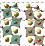
\includegraphics{../floats/nn_nt_tf_rlx/thin_film_nn_nt.pdf}
    };
    \draw (23mm,   16mm) node [coordinate] (nt1) {};
    \draw (23mm,    8mm) node [coordinate] (nt2) {};
    \draw (23mm,  -10mm) node [coordinate] (nt3) {};
    \draw (-23mm,  16mm) node [coordinate] (nb1) {};
    \draw (-23mm,   8mm) node [coordinate] (nb2) {};
    \draw (-23mm, -10mm) node [coordinate] (nb3) {};
\end{tikzpicture}

				\caption{Propriedades da estrutura cristalina dos filmes finos de \ce{NaNbO3} (esquerda) e \ce{NaTaO3} (direita).\label{fig:thin_film_nn_nt}}
			\end{figure}
		\end{column}
		\begin{column}{0.166666667\textwidth}
			\begin{tabular}{l}
				\toprule
				\multicolumn{1}{c}{\ce{NaTaO3}}\\\midrule
				\multicolumn{1}{c}{Superfície}\\
				\tikz[remember picture,overlay]{\node [anchor=west, shift={(-3.5mm, 1.5mm)}] (lista_nt1) {};}$\Delta \overline{d_{\ce{Ta-O}}} = \SI{-2.3}{\percent}$\\
				$P_L = \SI{84}{\percent}$\\\midrule
				\multicolumn{1}{c}{Subsuperfície}\\
				\tikz[remember picture,overlay]{\node [anchor=west, shift={(-3.5mm, 1.5mm)}] (lista_nt2) {};}$\Delta \overline{d_{\ce{Ta-O}}} = \SI{+2.1}{\percent}$\\
				$\Delta_d = \SI{3}{\percent}$\\\midrule
				\multicolumn{1}{c}{Interna}\\
				\tikz[remember picture,overlay]{\node [anchor=west, shift={(-3.5mm, 1.5mm)}] (lista_nt3) {};}$\Delta \overline{d_{\ce{Ta-O}}} = \SI{-0.1}{\percent}$\\
				$\Delta_d = \SI{0.3}{\percent}$\\\bottomrule
			\end{tabular}
		\end{column}\hspace{5mm}
	\end{columns}
	\begin{tikzpicture}[remember picture,overlay]
		\path (nt1) edge [arrow, out=0, in=180] (lista_nt1);
		\path (nt2) edge [arrow, out=0, in=180] (lista_nt2);
		\path (nt3) edge [arrow, out=0, in=180] (lista_nt3);
		\path (nb1) edge [arrow, out=180, in=0] (lista_nb1);
		\path (nb2) edge [arrow, out=180, in=0] (lista_nb2);
		\path (nb3) edge [arrow, out=180, in=0] (lista_nb3);
	\end{tikzpicture}
	\begin{equation*}
		\scriptstyle{P_L = \frac{\theta}{\SI{180}{\degree}};\; \Delta_d = \frac{1}{6} \sum^{6}_{i=1} \frac{|d_{\ce{Nb-O}\, i} - \overline{d_{\ce{Nb-O}}}|}{\overline{d_{\ce{Nb-O}}}};}
	\end{equation*}
\end{frame}
\begin{frame}{\texorpdfstring{\ce{NaNbO3}}{NaNbO3} \textit{vs.} \texorpdfstring{\ce{NaTaO3}}{NaTaO3}: Densidade de Estados}
	\begin{columns}
		\begin{column}{.5\textwidth}
			\begin{figure}[t]
				\centering
				\includegraphics{../floats/pdos_nn_nt_tf/pdos_rlx_nn_nt_surface.pdf}
				\caption{DOS projetada dos filmes finos em estado fundamental.\label{fig:pdos_rlx_nn_nt_surface}}
			\end{figure}	
		\end{column}
		\begin{column}{.5\textwidth}
			\begin{itemize}
				\item Mesma clivagem de duas ligações equatoriais \ce{M-O} gera níveis de superfície $d_{x^2-y^2}$;
				\item Níveis \ce{Ta} $5d_{x^2-y^2}$ completamente preenchidos no meio da banda proibida $\to$ rearranjo atômico \alert{mais intenso} estabilizou mais os níveis de superfície;
				\item Níveis \ce{Nb} $4d_{x^2-y^2}$ parcialmente preenchidos, hibridizados com a banda de condução $\to$ rearranjo atômico \alert{menos intenso} requeriu metalização;
				\item Relação com eletronegatividade;
			\end{itemize}
		\end{column}
	\end{columns}
\end{frame}
\begin{frame}{\texorpdfstring{\ce{NaNbO3}}{NaNbO3} \textit{vs.} \texorpdfstring{\ce{NaTaO3}}{NaTaO3}: Resposta à Tensão Biaxial}
	\begin{itemize}
		%\item \ce{NaTaO3}: redução dos parâmetros de rede afasta níveis de superfície da banda de condução e reduz DOS;
		%\item \ce{NaNbO3}: redução dos parâmetros de rede apenas reduz DOS;
		\item Em comum: compressão reduz $P_L$ e aumenta $\Delta_d$, tração aumenta $P_L$ e diminui $\Delta_d$ até deformação crítica;
		\item Diferenças: $P_L$ dos \ce{TaO4} alto $\to$ distorção dos \ce{TaO6} ocorre em \alert{trações menores} que em \ce{NbO6};
	\end{itemize}
	\begin{figure}[t]
		\centering
		\includegraphics{../floats/geometry_tf_nt_nn/nn_nt_pl_baur_strain_evolution.pdf}
		\caption{Índices de planaridade (superfície) e de deformação (subsuperfície e região interna) dos filmes finos.\label{fig:pl_baur_strain_evolution_NTOvsNNO}}
	\end{figure}
	\begin{equation*}
		\scriptstyle{P_L = \frac{\theta}{\SI{180}{\degree}};\; \Delta_d = \frac{1}{6} \sum^{6}_{i=1} \frac{|d_{\ce{Nb-O}\, i} - \overline{d_{\ce{Nb-O}}}|}{\overline{d_{\ce{Nb-O}}}};}
	\end{equation*}
\end{frame}
\begin{frame}{Evolução Comparada Da Estrutura Eletrônica: Compressão}
	\begin{columns}
		\begin{column}{.5\textwidth}
			\begin{figure}[t]
				\centering
				\includegraphics{../floats/pdos_nn_nt_tf/pdos_c5_nn_nt_surface.pdf}
				\caption{DOS projetada da camada superficial do filme fino sob tensão $\epsilon = -5\%$.\label{fig:pdos_c5_nn_nt_surface}}
			\end{figure}
		\end{column}
		\begin{column}{.5\textwidth}
			\begin{itemize}
				\item Em comum: compressão \alert{aumenta} o tamanho de banda proibida;
				\item \ce{NaNbO3}: níveis de superfície hibridizados com a banda de condução, diminui DOS;
				\item \ce{NaTaO3}: níveis de superfície isolados que adentram a banda proibida, diminui DOS;
			\end{itemize}
		\end{column}
	\end{columns}
\end{frame}
\begin{frame}{Evolução Comparada Da Estrutura Eletrônica: Tração}
	\begin{columns}
		\begin{column}{.5\textwidth}
			\begin{figure}[t]
				\centering
				\includegraphics{../floats/pdos_nn_nt_tf/pdos_t5_nn_nt_surface.pdf}
				\caption{DOS projetada da camada superficial do filme fino sob tensão $\epsilon = 5\%$.\label{fig:pdos_t5_nn_nt_surface}}
			\end{figure}
		\end{column}
		\begin{column}{.5\textwidth}
			\begin{itemize}
				\item Em comum: tração \alert{diminui} o tamanho da banda proibida;
				\item \ce{NaNbO3}: níveis de superfície hibridizados com a banda de condução, aumento da DOS;
				\item \ce{NaTaO3}: níveis de superfície isolados que se aproximam da banda de condução, aumento da DOS;
			\end{itemize}			
		\end{column}
	\end{columns}
\end{frame}
